\newpage
\section{Emptying a partition of all cards}
\genHeader
\hypertarget{sec:emptyPartition}{}

The next SDM we'll build should \emph{empty} a partition of all its cards by removing every card within it. To do this, we obviously need a construct for
repeating the action for all cards in the partition (Fig.~\ref{fig:goal_empty}). In SDM, this is \note{For Each} accomplished via a \emph{For Each} story node.
A \emph{for each} story node performs the specified actions for \emph{every} match in its pattern.

\vspace{0.5cm}

\begin{figure}[htbp]
	\centering
  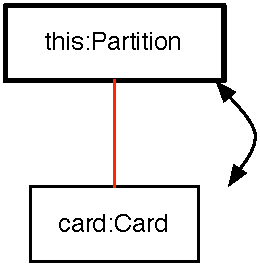
\includegraphics[width=0.25\textwidth]{empty.pdf}
	\caption{Emptying a partition of every card}
	\label{fig:goal_empty}
\end{figure}
\FloatBarrier

\vspace{0.5cm}
\begin{itemize}
\item[$\blacktriangleright$] Select a link below to begin this SDM.
\end{itemize}

\begin{center} {$\triangleright$ \hyperlink{emptyPartition vis}{Emptying a Partition: The visual syntax}}%
\\ \vspace{0.5cm}
{$\triangleright$ \hyperlink{emptyPartition tex}{Emptying a Partition: The textual syntax} }\end{center} 


\newpage
\subsection{Implementing empty}
\visHeader
\hypertarget{emptyPartition vis}{}

\begin{itemize}
\vspace{0.5cm}

\item[$\blacktriangleright$] To create a \emph{for each} story node in EA, create the initial diagram and start node for the method \texttt{Partition::empty},
then \emph{quick create} an activity node choosing \texttt{ForEach} as its type (Fig.~\ref{fig:sdm_foreach}). A \emph{for each} story node is visualised as a
double node to indicate potential repetition.

\vspace{1cm}

\begin{figure}[htbp]
\begin{center}
  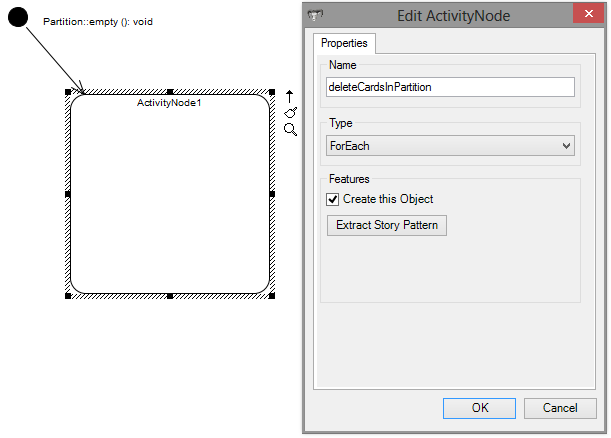
\includegraphics[width=0.9\textwidth]{ea_forEach}
  \caption{A for each loop in SDM.}  
  \label{fig:sdm_foreach}
\end{center}
\end{figure}

\vspace{1cm}

\item[$\blacktriangleright$] Next, complete the story pattern as indicated in Fig.~\ref{fig:sdm_end}. Please note that the \texttt{card} that is deleted in each match
is unbound, and both the \texttt{card} and link to \texttt{this} are set to \texttt{destroy}. Even more important, notice that the guard that terminates the for
each story node has an \texttt{[end]} guard. Indeed, a \emph{for each} story node \emph{must} have an end activity edge which is taken when all matches for the
story pattern have been handled.

\pagebreak

\begin{figure}[htbp]
\begin{center}
  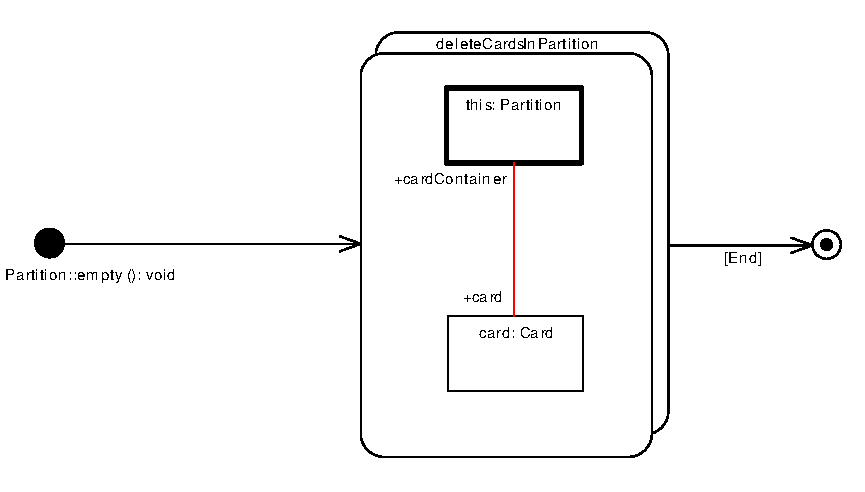
\includegraphics[width=0.9\textwidth]{ea_completeActivityEmptyCards.pdf}
  \caption{Complete story pattern with \texttt{[end]} guard.}  
  \label{fig:sdm_end}
\end{center}
\end{figure}

\fancyfoot[R]{ $\triangleright$ \hyperlink{sec:invertCard}{Next SDM} } \item[$\blacktriangleright$] Done! That's all we needed to do to specify a repeating
action. Pretty simple, eh? Inspect Figs. \ref{fig:emptyControlFlow} and \ref{fig:emptyPattern} to see how this is implemented textually.

\end{itemize}



\newpage
\hypertarget{emptyPartition tex}{}
\subsection{Implementing empty}
\texHeader

\begin{itemize}
 
\item[$\blacktriangleright$] To initialize your new control flow, you can once again take advantage of eMoflon's auto completion. Inside the
\texttt{empty} declaration, press  \texttt{Ctrl + Space} and select
\texttt{forEach} from the menu (Fig.~\ref{eclipse:typeCompletion}).

\vspace{1cm}

\begin{figure}[htpb]
\begin{center}
  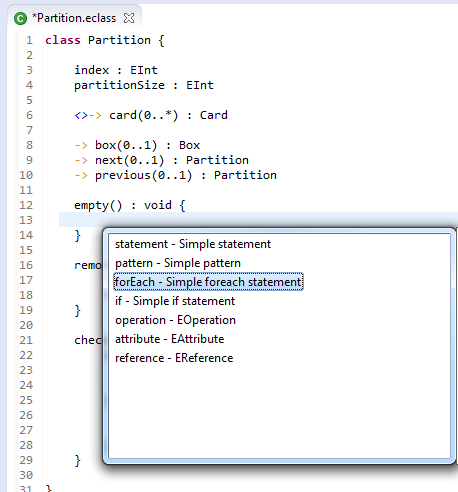
\includegraphics[width=0.7\textwidth]{eclipse_emptyTypeCompletion}
  \caption{eMoflon's auto completion}
  \label{eclipse:typeCompletion}
\end{center}
\end{figure}

\vspace{1cm}

\item[$\blacktriangleright$] Create a single pattern, \texttt{deleteCardsInPartition}. Remove the suggested second pattern as you only need to complete the
deletion -- no extra steps are required in this simple case!

\item[$\blacktriangleright$] Your activity should now resemble Fig.~\ref{eclipse:emptyControlFlow}.

\clearpage

\begin{figure}[htpb]
\begin{center}
  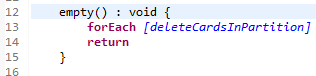
\includegraphics[width=0.5\textwidth]{eclipse_emptyControlFlow}
  \caption{Control flow for \texttt{partition.empty()}}
  \label{eclipse:emptyControlFlow}
\end{center}
\end{figure}

\item[$\blacktriangleright$] While similar to \texttt{removeCard} (Fig.~\ref{eclipse:deleteReference}), this new pattern will go one step further by requesting
a full destruction of \texttt{card}, instead of just deleting the link between the object variables. This means that in addition to destroying the link between
the partition and \texttt{card}, we need to destroy the object variable \texttt{card} as well.

\item[$\blacktriangleright$] Create a \texttt{@this} object variable, and delete its link to \texttt{card} via \syntax{-- -> card:card} Then create another
object variable \texttt{card}, deleting it by prefixing its name with the same \texttt{`--'} operator.

\vspace{0.5cm}

\item[$\blacktriangleright$] Your pattern should now resemble Fig.~\ref{eclipse:emptyPattern}.

\vspace{0.5cm}

\begin{figure}[htpb]
\begin{center}
  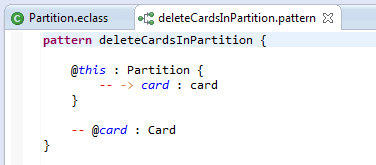
\includegraphics[width=0.6\textwidth]{eclipse_emptyPattern}
  \caption{Destroying both \texttt{card} and the link variable}
  \label{eclipse:emptyPattern}
\end{center}
\end{figure}

\vspace{0.5cm}

\item[$\blacktriangleright$] That's it! Look at you go\ldots you're just speeding through these SDMs now! To see how \texttt{empty} is specified in the visual
syntax, review Fig.~\ref{ea:sdm_end} from the previous section.

\vspace{0.5cm}

\item[$\blacktriangleright$] Although the Learning Box GUI does not have an explicit action that invokes this SDM, feel free to extend it and see your SDM in
action!

\end{itemize}
